\hypertarget{full-infall-simulations}{%
\chapter{Full infall simulations}\label{full-infall-simulations}}

\hypertarget{description-and-initial-results}{%
\section{Description and initial
results}\label{description-and-initial-results}}

With the equilibrated and merged initial conditions for both cuspy (CDM) and
cored (SIDM) galaxies, we now carry out our full simulations of the Sgr
infall.  We will consider \emph{three} mergers: the cuspy initial conditions
evolved using CDM microphysics, the cored initial conditions evolved with CDM
microphysics, and the cored initial conditions evolved with SIDM microphysics.
As before, we take \(\sigma / m\) = 10 cm\(^2\)/g in the SIDM case.  These
three mergers will be referred to as CDM/cusp, CDM/core, and SIDM
respectively.  By performing all three simulations, we will ideally be able to
identify whether certain discrepancies between the CDM/cusp and the SIDM runs
are the result of a cored initial profile or from the inclusion of
self-interactions.

For each merger, the infall is simulated for 10 Gyr, with snapshots saved
every 0.978 Gyr.  In Figure~\ref{fig:inits}, we show the positions of the
stars of Sgr in the orbital plane at several times for each merger.
Similarly, we show the positions of the Sgr dark matter particles in
% Figure~\ref{fig:darks}.

\begin{figure}
    \centering
    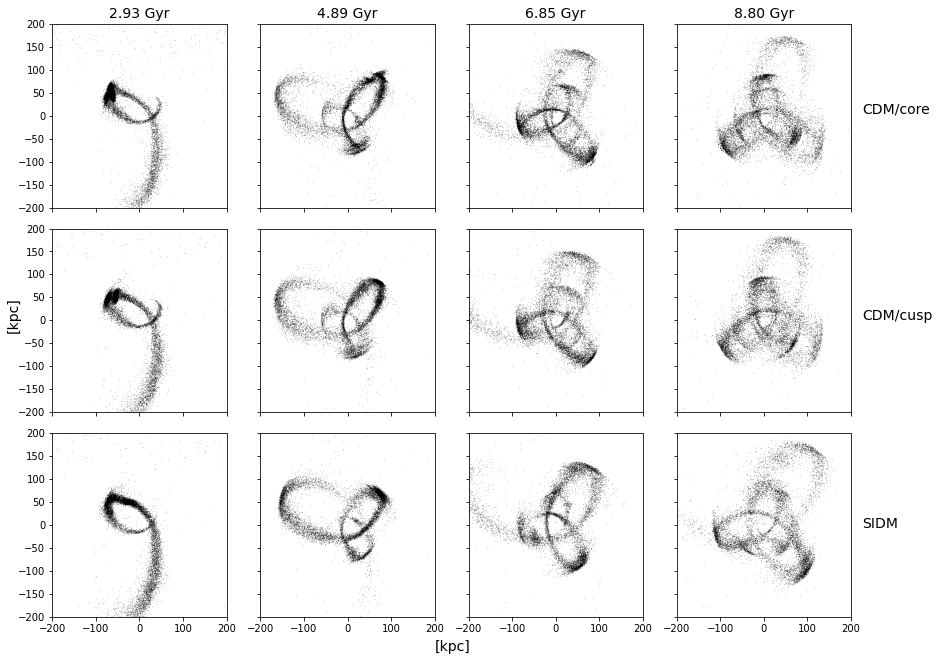
\includegraphics[width=0.9\linewidth]{figs/stars_bw.png}
    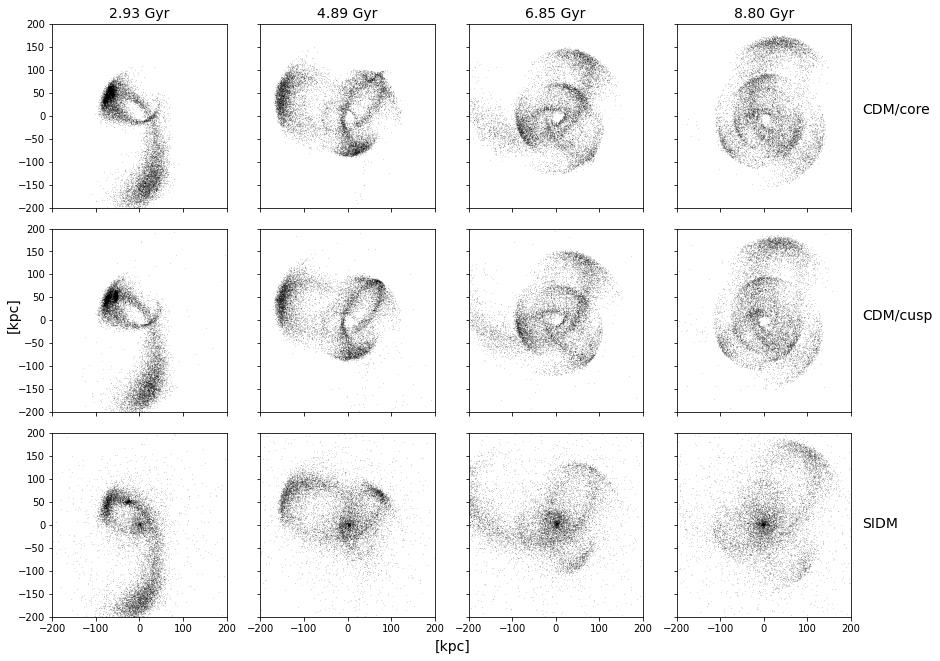
\includegraphics[width=0.9\linewidth]{figs/darks_bw.png}
    \caption{%
        Positions of Sgr stellar (top three rows) and dark matter (bottom
        three rows) particles at various times for all three of the considered
        mergers.  Each column denotes a different time; each row a different
        merger.
    }
    \label{fig:inits}
\end{figure}

Even from these plots, there are some interesting patterns to note. First, we
notice the development of a winding stream structure much like that reported
in~\cite{dierickx_predicted_2017} by around 6 to 7 Gyr in all three cases. We
can also note that the CDM/core and CDM/cusp are rather similar. There are some
discernible differences, but the general shape and size of the stream structure
is fairly similar throughout. 

There are quite marked differences between the SIDM and CDM cases, however.
The stream arms appear to be slightly rotated clockwise relative to the CDM
mergers, and the general shape of the inner structure is very different. These
differences are even more apparent when looking at the distribution of dark
matter. In the CDM mergers, the dark matter distribution appears to roughly
trace out the distribution of the stream. In the SIDM merger, however, the dark
matter distribution largely loses the shape of the stream, instead collapsing
inward toward the MW center.

We can also look at the density of particles in the orbital plane by performing
a two-dimensional histogram on the data in Figure~\ref{fig:inits}.  The result
is shown in Figure~\ref{fig:densities}.  The densities are integrated over the
axis perpendicular to the orbital plane.

\begin{figure}
    \centering
    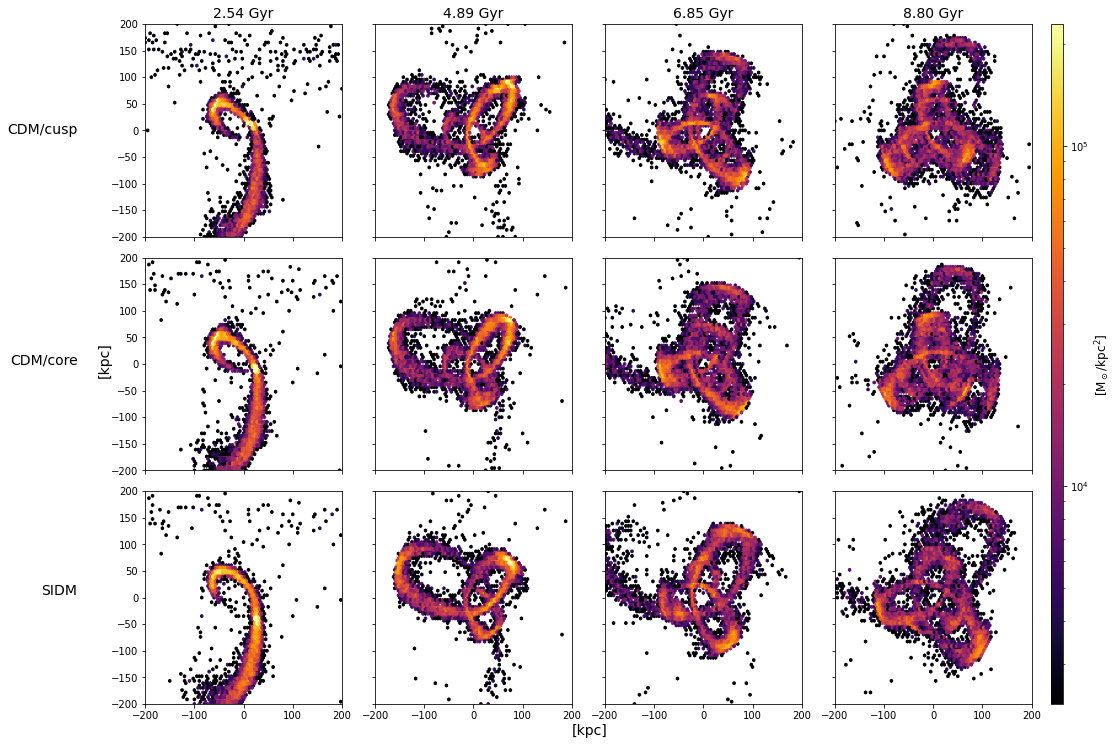
\includegraphics[width=0.9\linewidth]{figs/density_stars.png}
    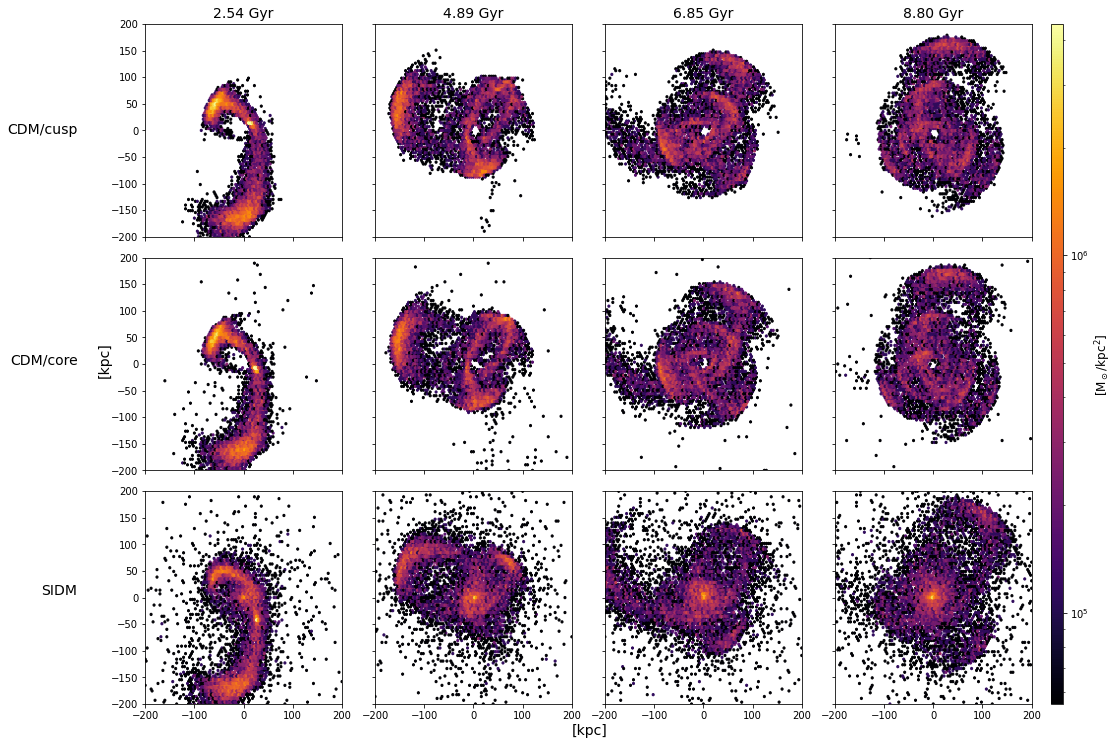
\includegraphics[width=0.9\linewidth]{figs/density_darks.png}
    \caption{%
        Two-dimensional density histogram of the stellar (top three rows) and
        dark matter (bottom three rows) Sgr particles at various times for
        each considered merger.  Densities are integrated over the axis
        perpendicular to the orbital plane.
    }
    \label{fig:densities}
\end{figure}

\hypertarget{identifying-the-sgr-progenitor}{%
\section{Identifying the Sgr
progenitor}\label{identifying-the-sgr-progenitor}}

A key part of analyzing these data is to understand the trajectory and
evolution of the Sgr progenitor in particular. As such, we desire a
method for successfully identifying the position of the Sgr progenitor
throughout its evolution. This is less straightforward than it may sound
because of the strong effects of tidal stripping. These mean that we
need to identify which particles are stripped or bound to the progenitor
at any given point and omit those particles which have been stripped
from our calculation of the progenitor position. In our tests, we tried
a few different methods which we will describe here.

The first method that we tried was to track bound versus unbound star
particles by counting particles as stripped once they exceeded a fixed radius
from the center of mass of those which are still bound.  The algorithm for
this is as follows.  We begin by counting the stellar particles within a
certain radius on the first snapshot to be ``bound''.  For each snapshot
after, we find the center of mass of the particles which are bound.  For each
bound particle, we compute its distance from the center of mass.  If this
exceeds the fixed stripping radius, we unmark the star as bound and continue.

As stated, this algorithm leaves has two parameters that can be tuned: the
initial stripping radius for the initial Sgr stellar positions and the fixed
stripping radius for all following snapshots. We found it useful to describe the
initial stripping radius instead in terms of the percentage of particles
that are initial counted as ``bound''. For example, we say that the we start
with the innermost 20\% of particles and proceed with a fixed radius of 20 kpc. 
effective for our mergers. The results of applying this algorithm to the
CDM/Cusp merger data with a few different choices of parameters can be seen in
Figure~\ref{fig:fixed_star}.

\begin{figure}
    \centering
    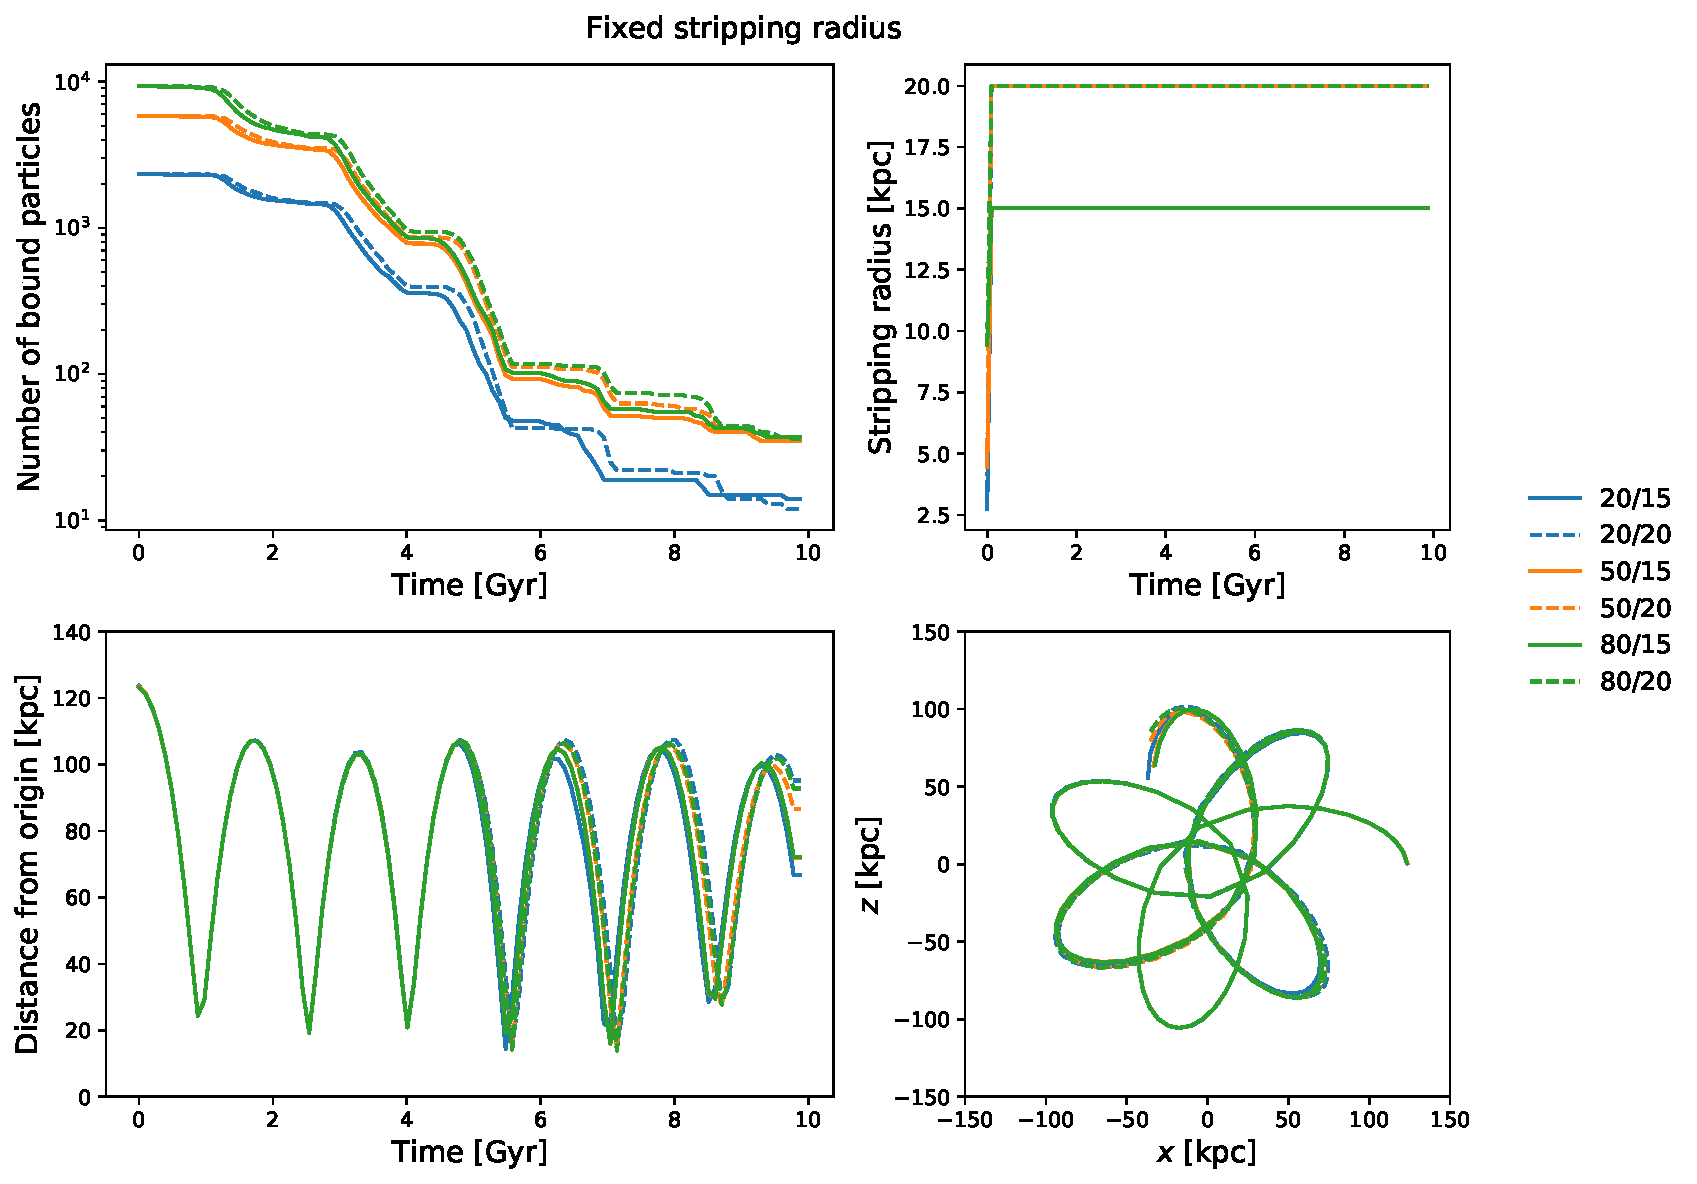
\includegraphics[width=0.9\linewidth]{figs/fixed_star.pdf}
    \caption{%
        Results of applying the ``fixed stripping radius''
        progenitor-identifying algorithm to the CDM/cusp merger data. Entries in
        the legend are given in the following format: ``a/b'' means that we
        started with the innermost ``a''\% of stellar particles and proceeded
        with a fixed stripping radius of ``b'' kpc.  In the upper left is the
        number of bound particles over time.  The upper right shows the
        stripping radius.  The bottom left shows the distance from the origin
        to the Sgr center of mass; an estimate of the MW-Sgr separation.  The
        bottom right shows the trajectory of the progenitor in the orbital
        plane.
    }
    \label{fig:fixed_star}
\end{figure}

This figure shows us that starting with too few of the initial particles (in
this case, 20\%) leads to very small numbers of bound particles at late times.
Further, it shows us that the trajectory of the progenitor can be somewhat
sensitive to the chosen algorithm parameters, especially at late times.

This algorithm appears to have two issues that we want to try to solve.
First, the actual size of the progenitor is expected to shrink with time, as
progressively more of the particles are stripped.  By using a fixed stripping
radius, we are not modeling the expected decay of the progenitor size.  The
second problem we encountered is that this method appears to leave us with
only $\mathcal{O}(10)$ bound particles after around 6 Gyr evolved.  As such,
we decided to explore modifications to the algorithm.

The first modification was to consider a decreasing stripping radius.  The
algorithm is very similar to before.  On the first snapshot, we count some
inner fraction of the particles to be ``bound'' and find the radius of this
ball of bound particles.  For the next snapshot, we strip any particles
which exceed this radius (times a constant).  \textit{However}, after
stripping away particles, we recompute the radius of the ball of the bound
particles, and reset the stripping radius equal to this. For each snapshot
following, we strip particles that are beyond this radius and recompute the
radius.  Over time, the stripping radius will decrease, modeling the
progressively decreasing size of the progenitor.  However, these modifications
tend to make the algorithm a bit \textit{too} aggressive, with it stripping
away all the particles in some cases.  We introduced a minimum stripping
radius such that the algorithm would choose the maximum of the given minimum and
the computed radius, but we found that the behavior in this case reduced to that
of the fixed-radius algorithm. The results of this decaying stripping radius are
shown in Figure~\ref{fig:decay_star}, with a minimum allowed stripping radius
of 8 kpc.

\begin{figure}
    \centering
    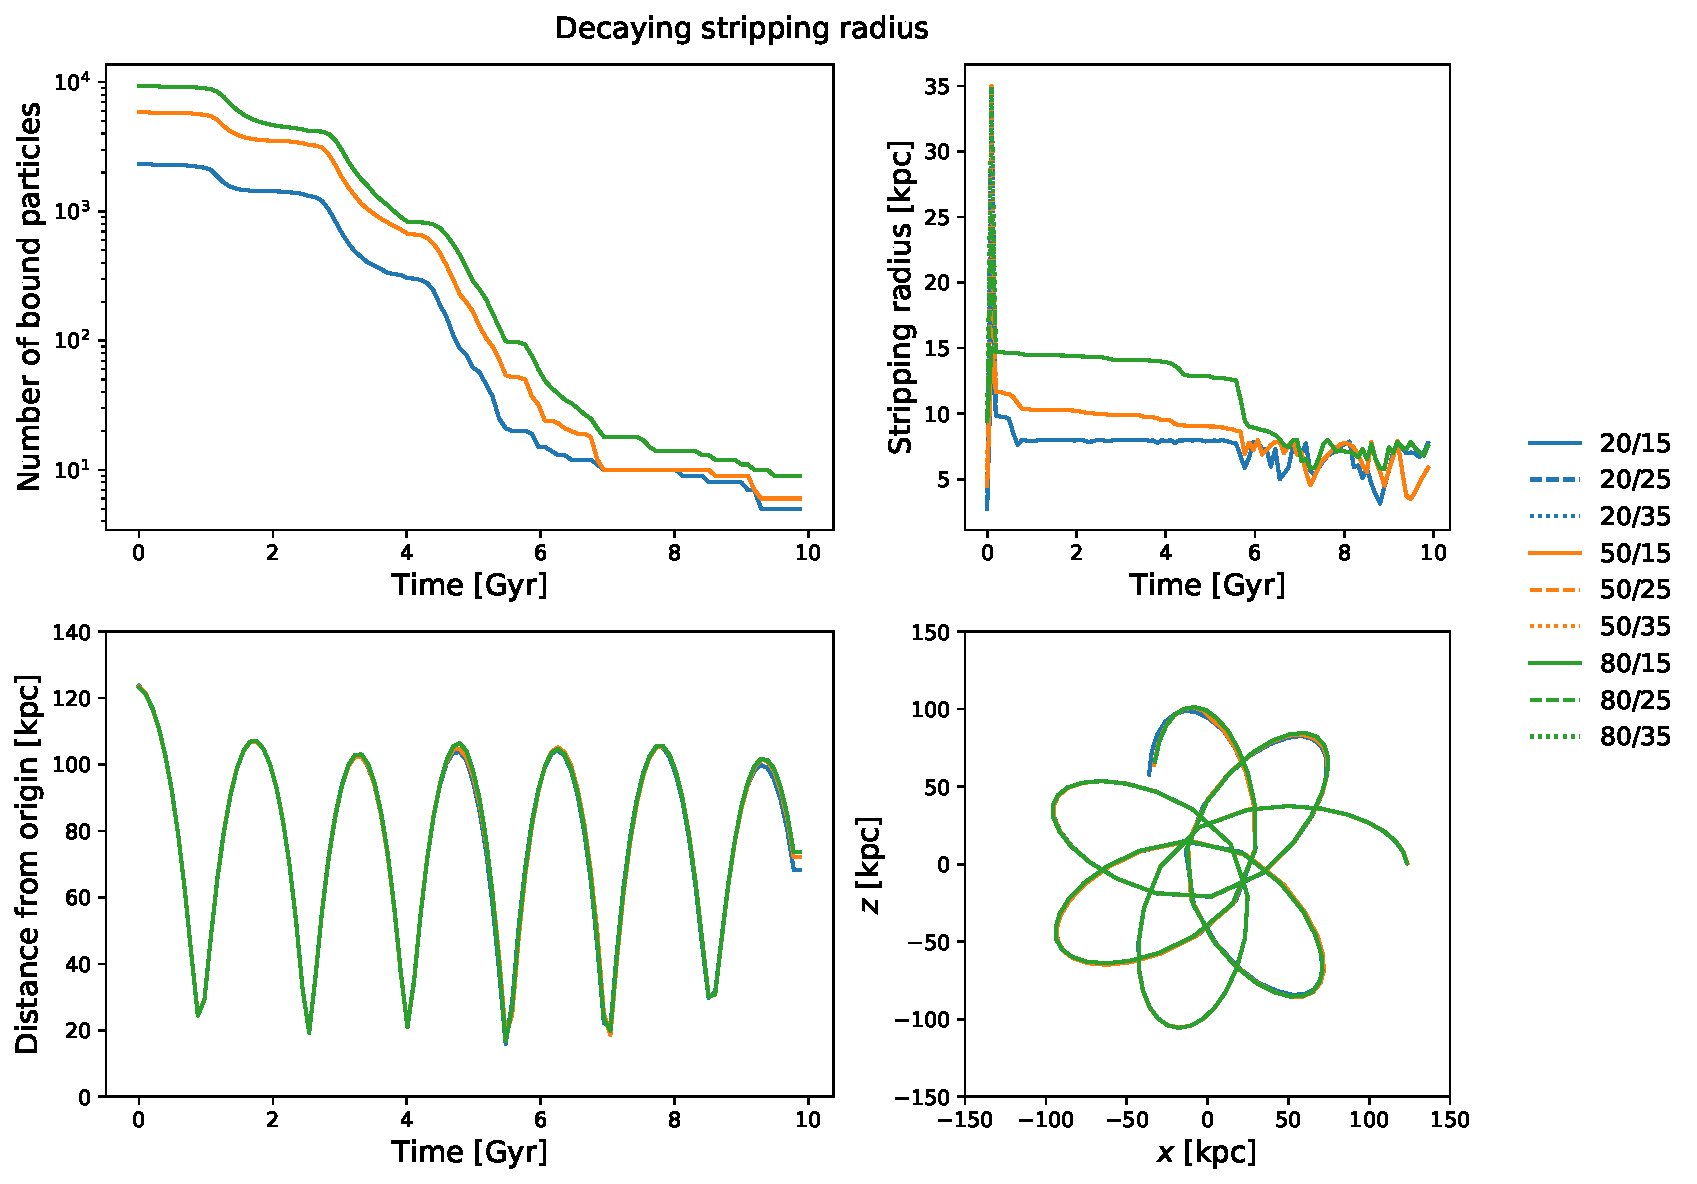
\includegraphics[width=0.9\linewidth]{figs/decay_star.pdf}
    \caption{%
        Results of applying the ``decaying stripping radius''
        progenitor-identifying algorithm to the CDM/cusp merger data with a
        minimum stripping radius of 8 kpc.  Plots have same meaning as in
        Figure~\ref{fig:fixed_star}.
    }
    \label{fig:decay_star}
\end{figure}

As can be seen in the figure, this algorithm leads to very aggressive stripping.
No matter the initial conditions, the desired stripping radius falls
\textit{very} quickly. For all considered parameter combinations, the desired
stripping radius fell below 8 kpc before the 6 Gyr mark, at which point the
algorithm will just default to using a fixed 8 kpc stripping radius. This
indicates that these changes are simply too aggressive and, when bundled with a
minimum stripping radius, is effectively equivalent to the fixed stripping
radius scheme.

One possible reason that it becomes too aggressive is because the actual
size of the progenitor is not monitonically decreasing.  Rather, its size
fluctuates over the course of the orbit, becoming quite compressed and small
near the pericenter and a bit more spread out and large near the apocenter.
These effects are modeled by the King formula for the tidal radius (todo cite
King) as given in~\cite{dierickx_predicted_2017}:
\begin{equation} \label{eq:king_radius}
    r_t = r \left[ \frac{1}{2} 
    \frac{M_{\text{Sgr}(<r_t)}}{M_{\text{MW}(<r)}} \right]^{1/3},
\end{equation}
where $M_{\text{gal}}(<r)$ is the enclosed halo mass in galaxy ``gal'' within
radius $r$ of the center of mass of the galaxy, $r$ is the distance between
the Milky Way and Sgr centers of mass, and $r_t$ is the tidal radius.  For a
given snapshot, then, we can compute the tidal radius according to this
formula by subtracting $r_t$ from both sides and using a simple root finder to
identify the $r_t$ which solves the equation.  We then strip any particles
which are farther than $r_t$ away from the center of mass of the progenitor at
the current time. The results of using the King tidal radius are shown in
Figure~\ref{fig:king_star}. Again, we pair this algorithm with a minimum
stripping radius of 8 kpc.

\begin{figure}
    \centering
    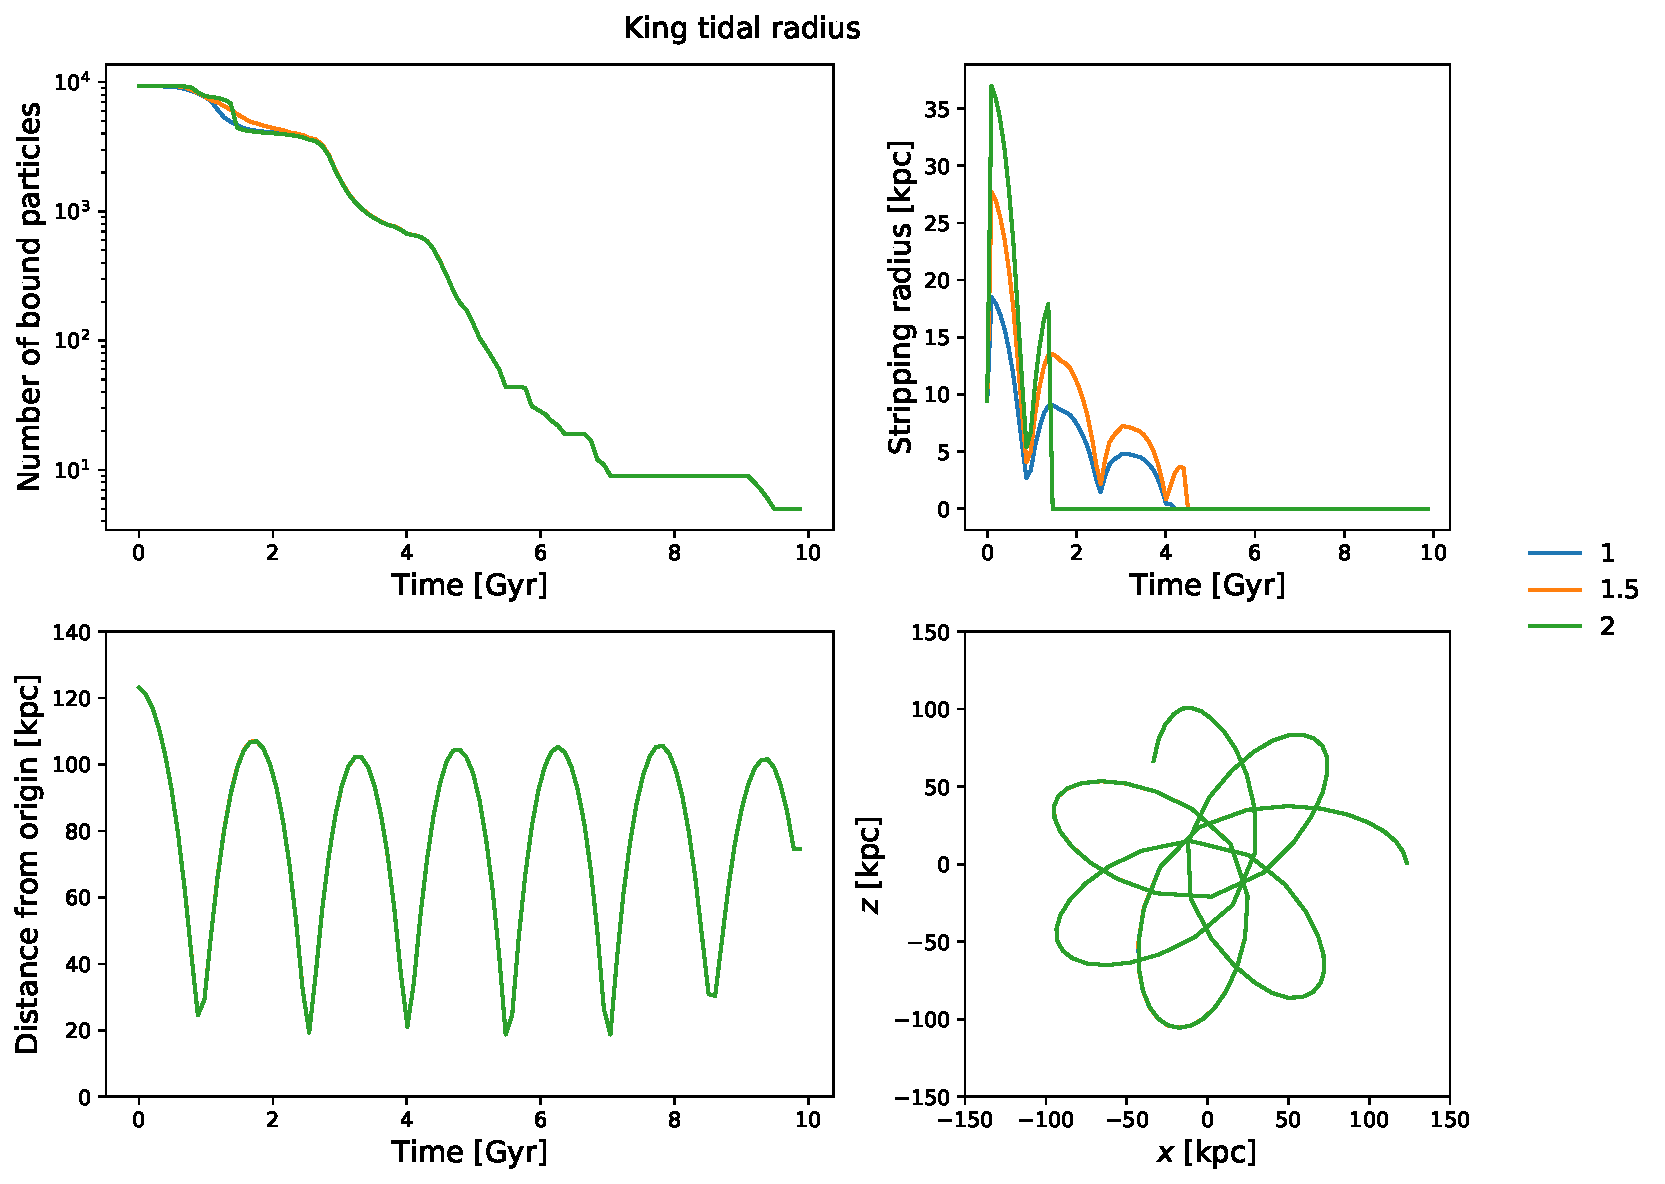
\includegraphics[width=0.9\linewidth]{figs/king_star.pdf}
    \caption{%
        Results of using the ``King tidal radius'' progenitor-identifying
        algorithm on the CDM/cusp merger data with a minimum stripping radius of
        8 kpc. The legend entries correspond to a fixed constant multiplied
        against the tidal radius before performing stripping. Plots again have
        the same meaning as in Figure~\ref{fig:fixed_star}.
    }
    \label{fig:king_star}
\end{figure}

Yet again, this algorithm appears to simply be too aggressive. In all cases, the
tidal radius quickly dips below the minimum stripping radius of 8 kpc. Further,
the algorithm appears to be somewhat unstable, defaulting to a recommended
radius of just \textit{zero} beyond a certain threshold. When this occurs, the
algorithm defaults to a fixed stripping radius equal to the minimum. Again,
then, this algorithm offers no improvements over the fixed radius.

At this point, it seems like the issue of too few bound particles at late times
may be a problem related to our relatively small number of Sgr stellar particles
instead of a problem with the algorithms themselves.  As such, we decided to
try to use the fixed algorithm but using both stellar \textit{and} dark matter
particles.  The result on the CDM/cusp data is shown in
Figure~\ref{fig:fixed_both}.

\begin{figure}
    \centering
    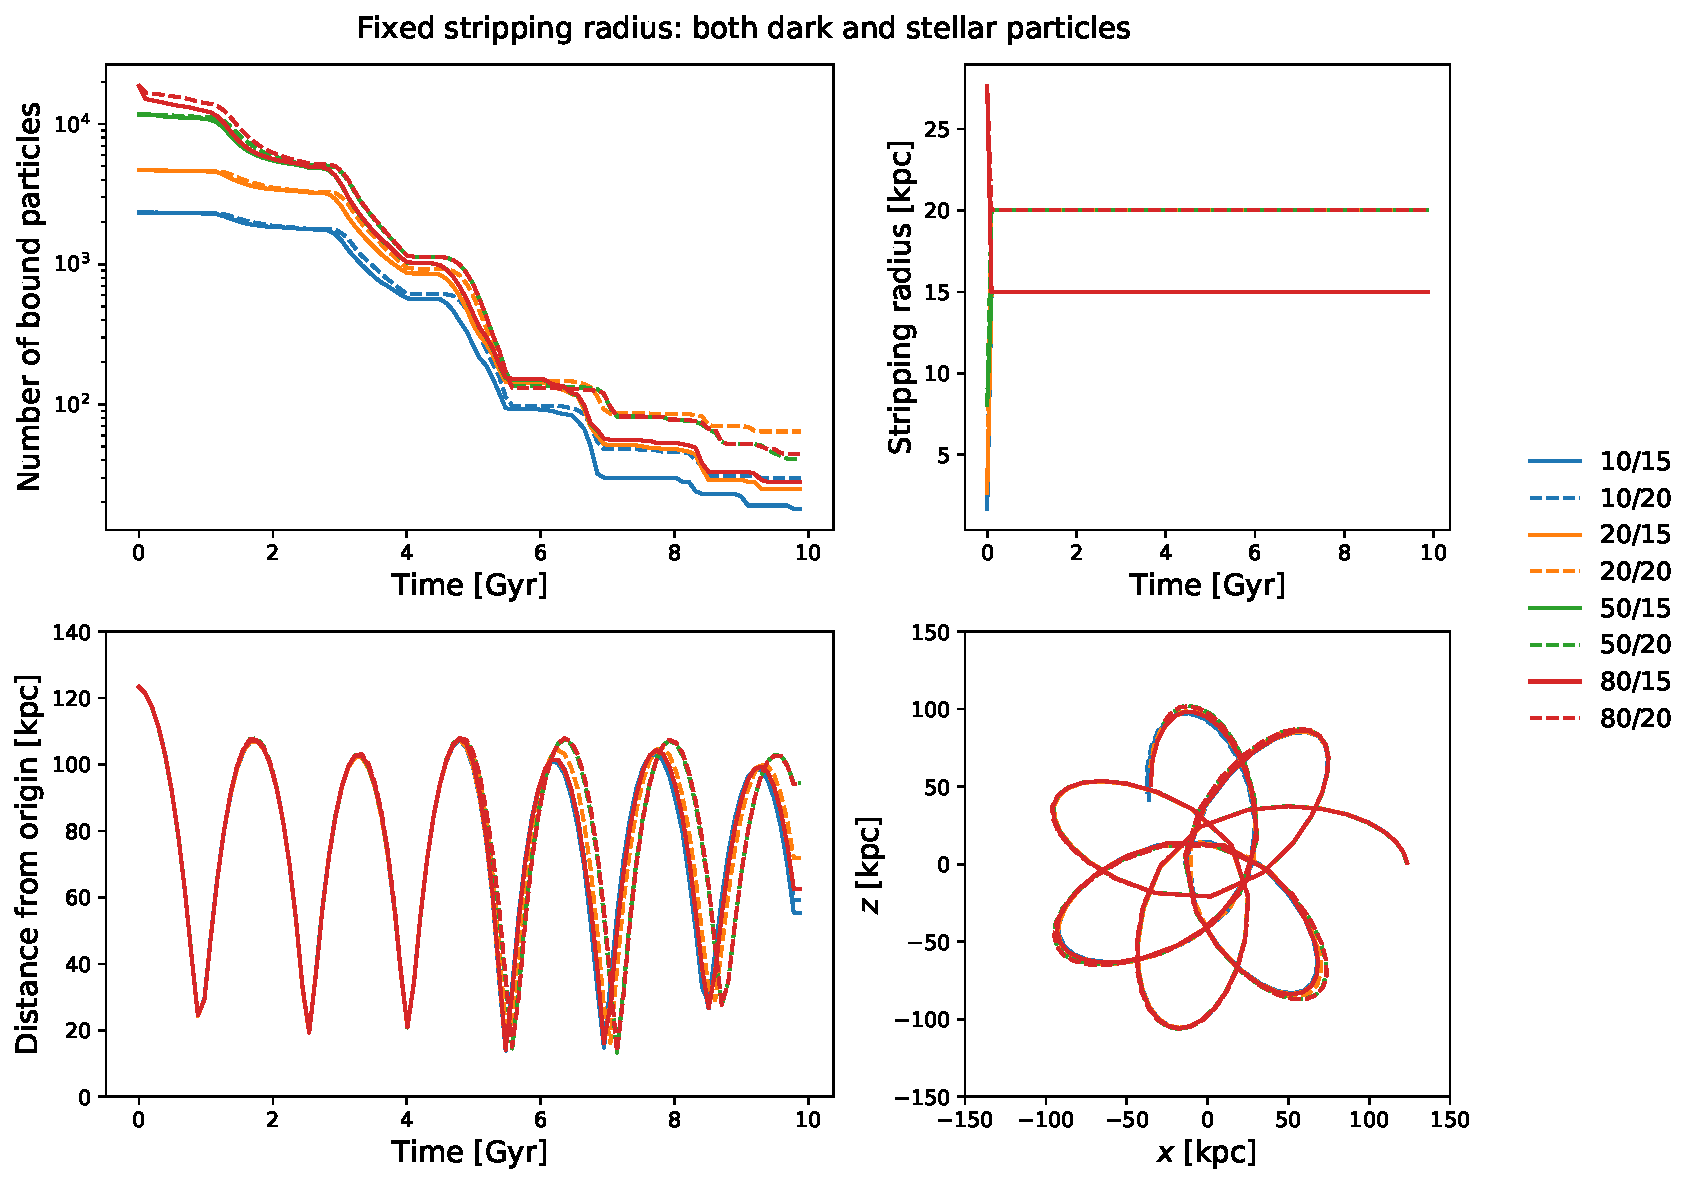
\includegraphics[width=0.9\linewidth]{figs/fixed_both.pdf}
    \caption{%
        Results of using the ``fixed stripping radius'' progenitor-identifying
        algorithm on the all particles in the CDM/cusp merger data. Plots and
        legend entries have the same meaning as in
        Figure~\ref{fig:fixed_star}.
    }
    \label{fig:fixed_both}
\end{figure}

This appears to yield promising results. We note that there are generally more
``bound'' particles at late times when using all particles than when only using
stellar ones, and that, aside from the ``50/20'' and ``80/20'' runs, the
resulting trajectories appear to be more robust to the algorithm parameters. As
such, we choose to move forward with this algorithm using the ``20/20''
parameters, as they appear to be consistent with the majority of the other
parameter choices and yield the most bound particles in the end. Using these
choices to identify the progenitor, we apply the algorithm to all three mergers.
The resulting data are shown in Figure~\ref{fig:all}.

\begin{figure}
    \centering
    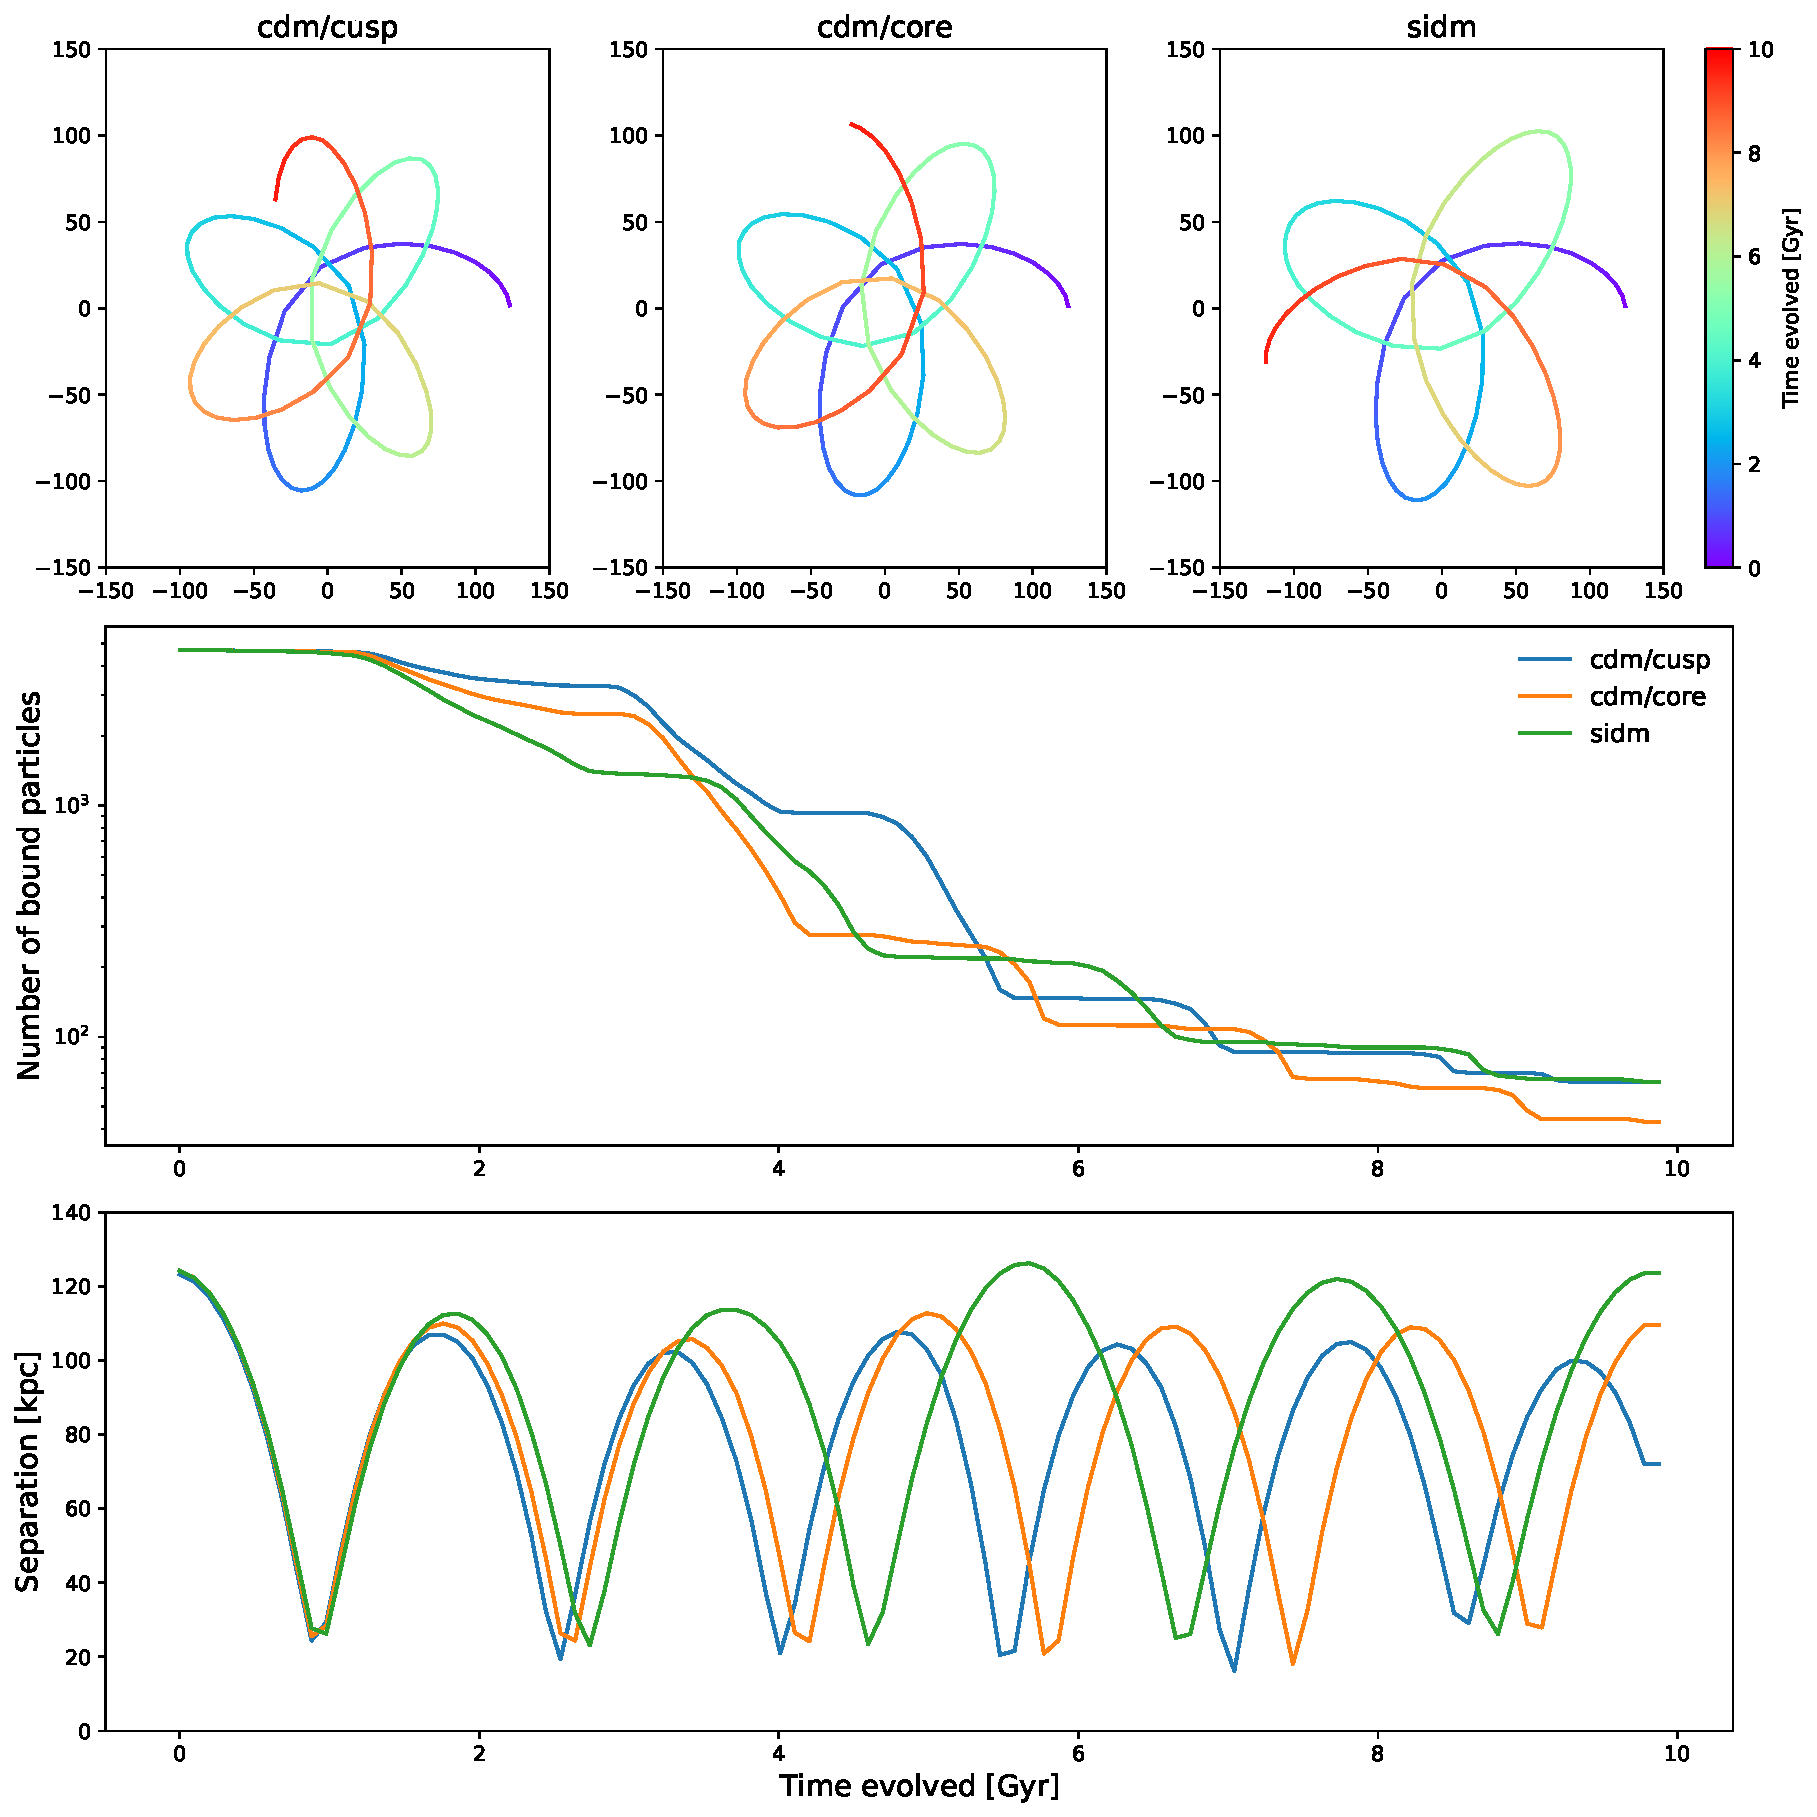
\includegraphics[width=0.9\linewidth]{figs/all_mergers_pretty.pdf}
    \caption{%
        Results of using the ``fixed stripping radius'' progenitor-identifying
        algorithm on all the particles in each of the mergers. We use the
        ``20/20'' algorithm parameters for all mergers, meaning that we start
        with the inner 20\% of particles and use a 20 kpc stripping radius. The
        top row shows the trajectory of the Sgr progenitor in the orbital plane
        for each merger. The middle row plot shows the number of bound particles
        over time. The bottom row plot shows the MW-Sgr separation over time.
    }
    \label{fig:all}
\end{figure}

The plots in this figure are evidence that SIDM microphysics may indeed have a
profound impact on the resulting trajectory of the Sgr satellite.  One
difference can be see in that the number of bound particles decreases much
more substantially at early times than either of the two CDM runs.  This could
be explained by considering that self-interactions provide a mechanism for
dark matter to free itself from shallow gravitational potential wells to which
collisionless dark matter would remain confined.

Looking at the MW-Sgr separation over time, it is immediately evident that the
cored profile yields a slightly longer orbital period, given the slowly
increasing distance between the apo- and pericenters of the CDM/cusp and
CDM/core orbits.  The inclusion of self-interactions appears to add to this
effect, with the CDM/cusp attaining six pericenters before the SIDM orbit is
able to reach a fifth.

One phenomenon showcased by the separation curves which is difficult to
understand is the lack of a consistent decay in the apocenters. We compare to
figure 6 of~\cite{dierickx_predicted_2017}, which shows a steadily decreasing
pericenter.  This is the expected behavior; as the Sgr progenitor orbits and
decays, we would expect it to lose energy and steadily fall inward.  This,
however, does not appear in our plots.  In fact, this phenomenon is
exacerbated in the SIDM merger, where the apocenter actually appears to
\textit{grow} after around 4 Gyr, reaching nearly 130 kpc at the 6 Gyr mark.
The mechanism by which this would occur is not yet understood.


\hypertarget{comparison-to-stream-data}{%
\section{Comparison to stream data}\label{comparison-to-stream-data}}

The last piece of the analysis that we will consider is a comparison to observed
data.  The data we will compare against comes from the second data release
(DR2) of the \textit{Gaia}
mission~\cite{lindegren_gaia_2018,gaia_collaboration_gaia_2018}, from which Sgr
stars have been identified by Ibata et al.~\cite{ibata_panoramic_2020} using the
\verb|STREAMFINDER|
algorithm~\cite{malhan_streamfinder_2018,malhan_ghostly_2018}. The resulting
dataset includes the \textit{Gaia} equatorial coordinates, proper motions,
magnitudes, and colors of 263,438 stars, along with an estimate of the distance
provided by the algorithm. They find their dataset to agree well with the Law
and Majewski 2010 model~\cite{law_sagittarius_2010}, barring a few small
deviations.

In~\cite{dierickx_predicted_2017}, the simulation was found to most closely
approximate the position of Sgr today at the fifth pericenter.  As such, we
consider the corresponding times in our mergers.  In our mergers, we find the
fifth pericenter to occur after 7.0 Gyr in the CDM/cusp merger, 7.4 Gyr in the
CDM/core merger, and 8.8 Gyr in the SIDM merger.

introduce the plot

\begin{figure}
    \centering 
    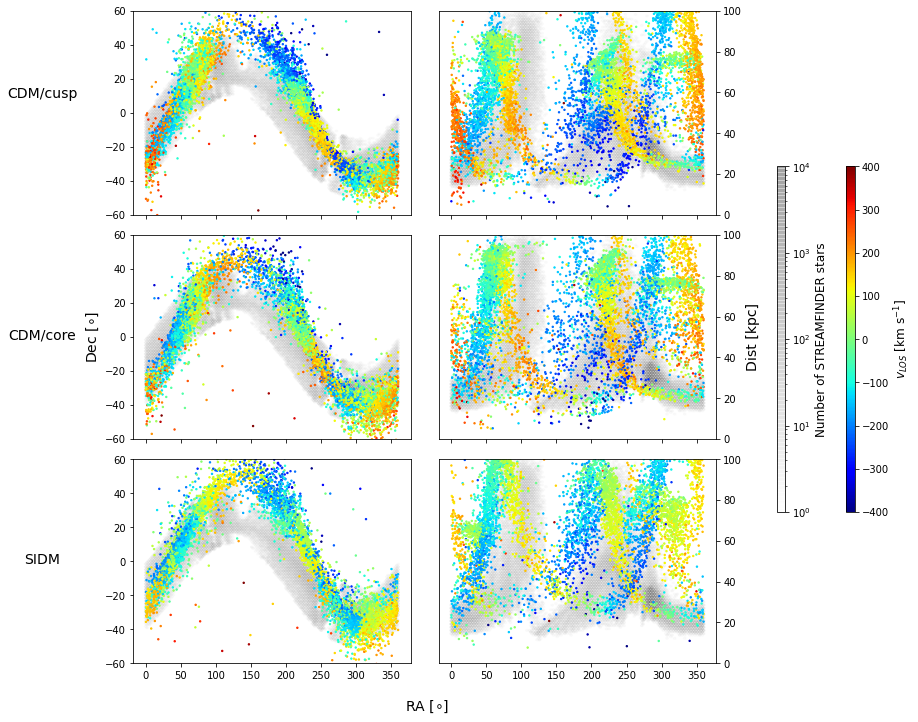
\includegraphics[width=1.0\linewidth]{figs/equatorial_streamfinder.png}
    \caption{%
        Equatorial coordinates for Sgr stellar particles at the time of the
        fifth pericenter for each merger. The density of STREAMFINDER particles
        is also shown in gray.
    }
    \label{fig:equatorial}
\end{figure}

talk about the plot


